This phase computes the adaptivity upper bound for a program $c$.
\\
Based on
% its 
$c$'s estimated dependency graph, $\progG({c})$ approximated above,
%
its adaptivity upper bound 
% Defined in Definition~\ref{def:prog_adapt} as 
%
is estimated as
the length of the longest finite walk over $\walks(\progG({c}))$ formally in Definition~\ref{def:prog_adapt}, 
and computed 
by Algorithm~\ref{alg:adapt}.
%
$\walks(\progG(c))$ represents the set of all finite walks on
% the estimated dependency graph for $c$
 $\progG({c})$.
Different from the finite walk on $\traceG(c)$, the $\kappa \in \walks(\progG(c))$ doesn't rely on the initial trace.
The occurrence time of every $v_i$ in $\kappa$'s vertices sequence is bound by 
an arithmetic expression $w_i$ where $(v_i, w_i) \in \progW(c)$ is $v_i$'s estimated weight.
Then its query length $\qlen(\kappa)$ and the estimated adaptivity $\progA(c)$ are both arithmetic expression as well.
%
They are formally defined as follows.
\begin{defn}[Finite Walk on estimated dependency graph ($\kappa$)].
  \label{def:prog_finitewalk}
  \\
  Given a program $c$'s estimated dependency graph 
  $\progG({c}) = (\progV(c), \progE(c), \progW(c), \progF(c))$, 
  a \emph{finite walk} $k$ in $\traceG({c})$ is
  a sequence of edges $(e_1 \ldots e_{n - 1})$ 
  for which there is a sequence of vertices 
  $(v_1, \ldots, v_{n})$ such that:
  \begin{itemize}
      \item $e_i = (v_{i},v_{i + 1}) \in \progE(c)$ for every $1 \leq i < n$.
      \item every vertex $v_i \in \progV(c)$,
      and $(v_i, w_i) \in \progW(c)$, 
       $v_i$ appears in $(v_1, \ldots, v_{n})$ at most 
    %   \wq{$\traceW({c})(\trace)$} 
    $w_i$
      times.  
  \end{itemize}
  %
  The length of $k$ is the number of vertices in its vertex sequence, i.e., $\len(k) = a$.
 \end{defn}

 \highlight{
  \begin{defn}[Finite Walk on estimated dependency graph ($\kappa$)].
    \label{def:prog_finitewalk}
    \\
    Given a program $c$'s estimated dependency graph 
    $\progG({c}) = (\progV(c), \progE(c), \progW(c), \progF(c))$, 
    a \emph{finite walk} $k$ in $\traceG({c})$ is
    a sequence of edges $(e_1 \ldots e_{n - 1})$ 
    for which there is a sequence of vertices 
    $(v_1, \ldots, v_{n})$ such that:
    \begin{itemize}
      \item 
        $e_i = (v_{i},w_i, v_{i + 1}) \in \progE(c)$ for every $1 \leq i < n$,
        and occurrence times of $e_i$ smaller than $w_i$.
      \item 
      every vertex $(v_i, w_i) \in \progV(c)$,
       $v_i$ appears in $(v_1, \ldots, v_{n})$ at most $w_i$ times. 
    \end{itemize}
    The length of $k$ is the number of vertices in its vertex sequence, i.e., $\len(k) = a$.
  \end{defn}
}
We abuse the notation $\walks(\progG(c))$ represents the walks over the estimated dependency graph for $c$.
Different from the walks on a program $c$'s semantics based graph,
 $k \in \walks(\traceG(c))$, 
$k \in \walks(\progG(c))$ doesn't rely on initial trace.
The occurrence times of every $v_i $ in $k$'s vertex sequence is bound by 
an arithmetic expression $w_i$ where $(v_i, w_i) \in \progV(c)$, is $v_i$'s estimated weight. 
% Notice here, for a walk in $\progG(c)$, the occurrence times of every vertex in vertices sequence, 
%  and its 
 The length of a finite walk $k \in \walks(\progG(c))$ is an arithmetic expression
 as well, i.e., $\len(k) \in \mathcal{A}_{in}$

Following the same procedure during defining the adaptivity in Section~\ref{sec:adaptivity}, we define
the \emph{query length} of a finite walk in the estimated graph, $\progG(c)$ as an arithmetic expression formally as follows.
\begin{defn}[Query Length of the Finite Walk on estimated dependency graph ($\qlen$)]
  \label{def:qlen}
  Given 
  a program $c$'s semantics-based dependency graph 
  $\progG({c}) = (\progV(c), \progE(c), \progW(c), \progF(c))$, 
   and a \emph{finite walk} $k \in \walks(\progG(c))$,
  The query length of $k$, $\qlen(k) \in \mathcal{A}_{in}$ 
  is the number of vertices which correspond to query variables in the vertices sequence of this walk $k$
  $(v_1, \ldots, v_{n})$ as follows, 
  \[
    \qlen(k) = |\big( v \mid v \in (v_1, \ldots, v_{n}) \land v \in \progF(c) \big)|.
  \]
  \end{defn}
  We estimate the adaptivity upper bound, $\progA(c)$ for a program $c$ as the maximum query length over all finite walks in its \emph{estimated dependency graph}, $\progG({c})$. 
\begin{defn}
[{estimated Adaptivity}]
\label{def:prog_adapt}
{
Given a program ${c}$ and its estimated dependency graph 
$\progG({c})$
%
the estimated adaptivity for $c$ is 
\[
\progA({c})
\triangleq \max
\left\{ \qlen(k) \ \mid \  k \in \walks(\progG(c))\right \}.
\]
}
\end{defn}

Similarly, the adaptivity bound $\progA(c)$ will also be a symbolic arithmetic expression over the input variables. With this symbolic expression we can prove the upper bound sound with respect to any initial trace, on its adaptivity in Definition~\ref{def:trace_adapt}.
\begin{thm}[Soundness of  \THESYSTEM]
  \label{thm:adaptfun_sound}
  For every program $c$, 
  its estimated adaptivity is a sound upper bound of its adaptivity.
   \[
   \forall \trace_0 \in \mathcal{T}_{0}(c), v \in \mathbb{N}^{\infty} \st 
\config{\progA(c), \trace_0} \earrow v \implies A(c)(\trace_0) \leq c
\] 
\end{thm}
The proof is in Appendix~\ref{apdx:adapt_soundness}.


Symbolic expressions as used in the weight  are great to express symbolic bounds but make the computation of 
a maximal walk harder. 
To compute $\progA(c)$ accurately and soundly, we develop an adaptivity computation algorithm named $\pathsearch$.
It combines the depth first search and breath first search strategies and computes a sound upper bound on $\progA(c)$.
$\pathsearch$ also involves another algorithm $\pathsearch_{\kw{SCC}}$ in \ref{alg:adaptscc} recursively, which finds the longest walk for a strong connected component (SCC) (SCC is the maximal strongly connected subgraph) of $\progG(c)$.
Theorem~\ref{thm:adaptalg_soundness} below formally describes the soundness of this algorithm with proof in Appendix~\ref{apdx:adaptalg_soundness}.
\begin{thm}[Soundness of $\pathsearch$]
    \label{thm:adaptalg_soundness}
    For every program $c$, given its \emph{Program-Based Dependency Graph} $\progG$,
    \[ \pathsearch(\progG({c})) \geq \progA(c).\]
\end{thm}

By Definition~\ref{def:prog_adapt}, the key point is to find the walks in the estimated dependency graph. 
We first discuss two challenges when we try to find the walks,
and then show that how we solve them using our algorithms.

\textbf{Non-Termination Challenge:}
% Moreover, b
One naive walk finding method is to simply traverse on this graph and decrease the weight of every node by one after every visiting. However, this simple 
traversing strategy leads to non-termination dilemma for most programs which we are interested in. 
Because the weight of each vertex in a program's estimated dependency graph,
which is an arithmetic expression containing input variables. 
In this sense, the simple traversing could never terminate when domain of the input variables isn't finite.
However, it is very common that the domain of program's input variables is infinite such as natural number $\mathbb{N}$, real number $\mathbb{R}$, or etc. As the simple while loop example program in Figure~\ref{fig:kadaptwhile_alg} with k adaptivity rounds, the input variable $k$ has domain $\mathbb{N}$.
% Analysis Results: $ \progA(\kw{whileRec}(k)) = 1 + k$
%
If we traverse on the estimated dependency graph, and decrease the weight of $x^3$ (the weight $k$ is symbolic) by one after every visit,
% We can simply adopt either a depth first strategy to estimate the adaptivity as the length of the longest weight path, as 
% in Algorithm~\ref{alg:overadp_alg}.
we will never terminate because we only know $k \in \mathbb{N}$.

\begin{figure}
    \centering
    {
    \small
    \begin{subfigure}{.4\textwidth}
    \begin{centering}
    $ 
    \begin{array}{l}
      \kw{whileSim(k)} \triangleq \\
      \clabel{ \assign{j}{k} }^{0} ;
      \clabel{ \assign{x}{\query(\chi[0])} }^{1} ; \\
          \ewhile ~ \clabel{j > 0}^{2} ~ \edo ~ \\
          \Big(
           \clabel{\assign{x}{\query(\chi[x]) }}^{3}  ; 
          \clabel{\assign{j}{j-1}}^{4}       \Big)
      \end{array}
    $
    \caption{}
    \end{centering}
    \end{subfigure}
    \quad
      \begin{subfigure}{.45\textwidth}
      \begin{centering}
      \begin{tikzpicture}[scale=\textwidth/22cm,samples=200]
    \draw[] (0, 7) circle (0pt) node
    {\textbf{$x^1: {}^{1}_{1}$}};
    \draw[] (0, 4) circle (0pt) node
    {{ $x^3: {}^{k}_{1}$}};
    % Counter Variables
    \draw[] (10, 7) circle (0pt) node {{$j^2: {}^{1}_{0}$}};
    \draw[] (10, 4) circle (0pt) node {{ $j^4: {}^{k}_{0}$}};
    %
    % Value Dependency Edges:
    \draw[ ultra thick, -latex, densely dotted,] (0, 4.2)  -- (0, 6.5) ;
    \draw[ ultra thick, -Straight Barb, densely dotted,] (2, 4.5) arc (150:-180:1);
    \draw[ thick, -Straight Barb] (11.3, 4.7) arc (150:-150:1);
    \draw[ thick, -latex] (10, 4.6)  -- (10, 6.5) ;
    % Control Dependency
    \draw[ thick,-latex] (1.5, 7)  -- (8, 7) ;
    \draw[ thick,-latex] (1.5, 4)  -- (8, 7) ;
    \draw[ thick,-latex] (1.5, 7)  -- (8, 4) ;
    \draw[ thick,-latex] (1.5, 4)  -- (8, 4) ;
    \end{tikzpicture}
    \caption{}
      \end{centering}
      \end{subfigure}
    }
    % \end{wrapfigure}
    % \end{equation*}
    \vspace{-0.4cm}
     \caption{(a) The simple k adaptivity rounds while loop example (b) The program-based dependency graph generated from $\THESYSTEM$.}
    \label{fig:kadaptwhile_alg}
    \end{figure}

To solve this non-termination challenge, we switch to another walk finding approach:
finding the longest path in the estimated dependency graph via depth first search and then use this path as the estimated longest walk.
Through a simple depth first search algorithm, we find the longest weighted path as the dotted arrow in Figure~\ref{fig:kadaptwhile_alg}(c),
$x^3: {}^k_1 \to x^1: {}^1_1 $.
Then, by summing up the weights on this path where the vertices have query annotations $1$, depth first search algorithm gives the adaptivity bound $k$.
This is a tight bound for this simple k adaptivity rounds example program.

\textbf{Approximation Challenge:}
% As in Definition~\ref{def:finitewalk}, w
% When we adopt a depth first strategy to search for the longest weighted path, and then use the path to approximate the adaptivity. 
However, this naive approximation via depth first searching over-approximates the adaptivity rounds largely in many cases.
It computes $\infty$ adaptivity upper bound for our $\kw{twoRounds}$ example program in Figure~\ref{fig:overview-example}, which has only $2$ adaptivity rounds.
% Look at the two-round example in overview, 
% it is easy to find that 
More specifically, the depth first searching finds the longest weighted path,
$x^3 : {}^{k}_{1} \to a^5 : {}^{k}_{0} \to l^6 : {}^{1}_{0}$.
Then, it computes the weighted length, $1 + k$.
If we use this path to approximate the longest finite walk, and weight of each vertex as
%  their visiting times, 
its visiting time, then we have a walk, $x^3 \to \cdots \to x^3 \to a^5 \to \cdots \to a^5 \to l^6$.
However, this isn't a qualified walk by our Definition~\ref{def:finitewalk}.
% then it isn't a qualified walk. 
% In the approximated walk, we have the vertices as $x^3 \to \cdots \to x^3 \to a^5 \to \cdots \to a^5 \to l^6$.
Because $l^6$ has weight $1$, it can only be visited as most once. In this sense,
% and this lead to 
% resulting in the restriction on 
% the maximum visiting time of 
% ,
% such that $x^3$ 
$x^3$ is only able to be visited at most once as well, because the only way to re-visit $x^3$ is through $l^6 \to a^5 \to x^3$.
%
Contradictory, $x^3$ is visited $k$ times in this approximated walk.
As a result,
% the with the weighted length $1 + k$. It is obviously
the weighted length of this path is $1 + k$, which
% which is 
over approximates 
% its 
this two rounds example program's adaptivity rounds, which is supposed to be $2$. 

%%%%%%%%%%%%%%%%%%%%%%%%%%%%%%%%%%%%%%%%%%%%%%%%%%%%%%%%%%%%%%%%%%%%%%%%%%%%%%%%%%%%%%%%%%%%%%%%%%%%%%%%%%%%%%%%%%%%%%%%%%%%%%%%%%%%%%%%%%%%%%%%%%%%%%%%%%
%%%%%%%%%%%%%%%%%%%%%%%%%%%%%%%%%%%%%%%%%%%%%%%%% INTRODUCTION OF THE COMBINED ADAPTIVITY COMPUTATION ALGORITHM: %%%%%%%%%%%%%%%%%%%%%%%%%%%%%%%%%%
%%%%%%%%%%%%%%%%%%%%%%%%%%%%%%%%%%%%%%%%%%%%%%%%%%%%%%%%%%%%%%%%%%%%%%%%%%%%%%%%%%%%%%%%%%%%%%%%%%%%%%%%%%%%%%%%%%%%%%%%%%%%%%%%%%%%%%%%%%%%%%%%%%%%%%%%%%
\textbf{Adaptivity Computation Algorithm}
To this end, we combine the 
% DFS and BFS algorithm 
depth first search and breath first search strategies in our longest walk estimation algorithm.
%
Our algorithm reduces the task of computing the longest walk into the computation of local adaptivity and the composition of
local adaptivity into global adaptivity.
%
We exploit the structure of the estimated dependency graph $\progG(c)$ for a program $c$: 
1). Partitioning the PDG of programs into its strongly connected components (SCCs) (SCCs are maximal strongly connected subgraphs).
2). Then, for each SCC, we compute an adaptivity bound
3). In the last, we compose these local bounds to an overall adaptivity bound.
%
$\pathsearch(c, \progG(c))$ algorithm in Algorithm~\ref{alg:adapt} arranges the estimated dependency graph $\progG(c)$ into SCCs ($\kw{SCC_1}, \cdots, \kw{SCC_n}$) and obtains the adaptivity local bound of each SCC from $\kw{\pathsearch_{SCC}(c, SCC_i)}$ algorithm in Algorithm~\ref{alg:adaptscc}.
Then $\pathsearch$ shrinks the estimated dependency graph into a directed acyclic graph (DAG) by reducing each SCC into a vertex with the weight equal to its adaptivity local bound.
In this way, it simply computes the length of the longest path over this DAG.

%%%%%%%%%%%%%%%%%%%%%%%%%%%%%%%%%%%%%%%%%%%%%%%%%%%%%%%%%%%%%%%%%%%%%%%%%%%%%%%%%%%%%%%%%%%%%%%%%%%%%%%%%%%%%%%%%%%%%%%%%%%%%%%%%%%%%%%%%%%%%%%%%%%%%%%%%%
%%%%%%%%%%%%%%%%%%%%%%%%%%%%%%%%%%%%%%%%%%%%%%%%% INTRODUCTION OF ADAPTIVITY COMPUTATION ALGORITHM 1: %%%%%%%%%%%%%%%%%%%%%%%%%%%%%%%%%%
%%%%%%%%%%%%%%%%%%%%%%%%%%%%%%%%%%%%%%%%%%%%%%%%%%%%%%%%%%%%%%%%%%%%%%%%%%%%%%%%%%%%%%%%%%%%%%%%%%%%%%%%%%%%%%%%%%%%%%%%%%%%%%%%%%%%%%%%%%%%%%%%%%%%%%%%%%
\paragraph*{The Adaptivity Computation Algorithm ($\pathsearch(c, \progG(c))$)}
\begin{algorithm}
    \caption{
    {Adaptivity Computation Algorithm ({$\kw{\pathsearch(c, \progG(c))}$})}
    \label{alg:adapt}
    }
    \begin{algorithmic}[1]
    \REQUIRE The program $c$, 
    Its estimated dependency graph: $\progG(c) = (\vertxs, \edges, \weights, \qflag)$
    \STATE {\bf init} 
    % \\
    % current node: $c$, 
    \\
    $q$: empty queue.
    % \\
    \\
    $\kw{adapt}$ : the adaptivity of this graph initialize with $0$.
    \\
    \STATE Find all Strong Connected Components (SCC) in $G$: $\kw{SCC_1}, \cdots, \kw{SCC_n}, 0 \leq n \leq |\vertxs|$, 
    \STATE {\bf for} every SCC: $\kw{SCC_i}$, compute its Adaptivity $\kw{SCC_i}$:
    \STATE \quad $\kw{adapt_{scc}[SCC_i] = \pathsearch_{scc}(c, SCC_i)}$;
    \STATE {\bf for} every $\kw{SCC_i}$:
    \STATE \qquad $q.append(\kw{SCC_i})$;
    \STATE \qquad $\kw{adapt_{tmp}} = 0$;
    \STATE \qquad {\bf while} $q$ isn't empty:
    \STATE \qquad \qquad $\kw{s} = q.pop()$;  \#\{take the top SCC from head of queue\}
    \STATE \qquad \qquad  $\kw{adapt_{tmp}}_0= \kw{adapt_{tmp}}$; \#\{record the adaptivity of last level\}
    \STATE \qquad \qquad  $\kw{SCC_{max}}$;  \#\{record the SCC with longest walk in this level\}
    % initialize cycle-adapt = 0.
    \STATE \qquad \qquad {\bf for} every 
    different SCC, $\kw{s'}$ connected by $\kw{s}$ by a directed edge from $\kw{s}$:
    \STATE \qquad \qquad \qquad {\bf if} $(\kw{adapt_{tmp}} < \kw{adapt_{tmp}}_0 + \kw{adapt_{scc}[s']})$:
    \STATE \qquad \qquad \qquad \qquad $\kw{adapt_{tmp}} = \kw{adapt_{tmp}}_0 + \kw{adapt_{scc}[s']}$; 
    \STATE \qquad \qquad \qquad \qquad $\kw{SCC_{max} = s'} $; \#\{update the SCC with the longest walk in this level\} 
    \STATE \qquad \qquad \qquad $q.append(\kw{SCC_{max}})$;
    \STATE \qquad $\kw{adapt} = \max(\kw{adapt}, \kw{adapt_{tmp}})$;    
    \RETURN $\kw{adapt}$.
    \end{algorithmic}
    \end{algorithm}
    %
    % it 
    At Line:3, this algorithm first finds all the SCCs of $\progG(c)$, $\kw{SCC_1}, \cdots, \kw{SCC_n}$
    where $0 \leq n \leq |\vertxs|$ by the standard Kosaraju’s algorithm, where each
    % Every SCC is a sub-graph of $\progG(c)$, where 
    $\kw{SCC_i} = (\vertxs_i, \edges_i, \weights_i, \qflag_i)$.
    % where $\kw{SCC_i} = (\vertxs_i, \edges_i, \weights_i, \qflag_i)$.
    Then, 
    it computes the adaptivity local bound on every $\kw{SCC_i}$
    % , which is a subgraph of the $\progG(c)$, 
    in line:4-5 by $\kw{\pathsearch_{SCC}(c, SCC_i)}$.
    We guarantee the soundness of the adaptivity local bound on an SCC by Lemma~\ref{lem:adaptalg_soundness_scc} with formal proof in Appendix~\ref{apdx:adaptalg_soundness}.
    The $\progG(c)$ is then shrunk into a directed acyclic graph where 
    % vertices are all the SCCs and edges are between every SCCs with their adaptivities as weights.
    $\kw{SCC_1}, \cdots, \kw{SCC_n}$ are all the vertices and the adaptivity local bounds are their weights.
    % , and directed edges are .
    There is an edge $s_i \to s_j$ in this shrank graph, as long as we can find an edge $v_i \to v_j \in \progE(c)$ such that $v_1 \in \vertxs_i$, $v_j \in \vertxs_j$ and $i \neq j$.
    % \\ 
    Then, we use the standard breath first search strategy to find the longest weighted path
    %  w.r.t. all the SCCs and their adaptivities.
    on this DAG and return this length as the adaptivity upper bound.
    \\
    We guarantee that 
    % this longest weighted path is a sound computation of the adaptivity on this,
    the length of this longest weighted path is a sound computation of the adaptivity for program $c$
    % as well as 
    and this longest weighted path is a sound computation of the finite walk having the longest query length 
    on $c$'s estimated dependency graph in Theorem~\ref{thm:adaptalg_soundness}
    in Appendix
    ~\ref{apdx:adaptalg_soundness}.
    %
If a program
$c$'s estimated dependency graph $\progG(c)$ is a DAG, then we prove that the adaptivity upper bound by Algorithm~\ref{alg:adapt} is tight formally in Theorem~\ref{thm:adaptalg_pcomplete} in Appendix~\ref{apdx:adaptalg_completeness}.

%%%%%%%%%%%%%%%%%%%%%%%%%%%%%%%%%%%%%%%%%%%%%%%%%%%%%%%%%%%%%%%%%%%%%%%%%%%%%%%%%%%%%%%%%%%%%%%%%%%%%%%%%%%%%%%%%%%%%%%%%%%%%%%%%%%%%%%%%%%%%%%%%%%%%%%%%%
%%%%%%%%%%%%%%%%%%%%%%%%%%%%%%%%%%%%%%%%%%%%%%%%% INTRODUCTION OF ADAPTIVITY COMPUTATION ALGORITHM 1: %%%%%%%%%%%%%%%%%%%%%%%%%%%%%%%%%%
%%%%%%%%%%%%%%%%%%%%%%%%%%%%%%%%%%%%%%%%%%%%%%%%%%%%%%%%%%%%%%%%%%%%%%%%%%%%%%%%%%%%%%%%%%%%%%%%%%%%%%%%%%%%%%%%%%%%%%%%%%%%%%%%%%%%%%%%%%%%%%%%%%%%%%%%%%
\paragraph*{Adaptivity Computation Algorithm on An SCC ($\kw{\pathsearch_{scc}(c, SCC_i)}$)}
\begin{algorithm}
  \caption{
  {Adaptivity Computation Algorithm on An SCC ({$\kw{\pathsearch_{scc}(c, SCC_i)}$})}
  \label{alg:adaptscc}
  }
  \begin{algorithmic}[1]
    \REQUIRE The program $c$, 
    An strong connected component of $\progG(c)$: $ \kw{SCC_i} = (\vertxs_i, \edges_i, \weights_i, \qflag_i)$
  % {\bf {$\kw{\pathsearch_{scc}(c, SCC_i)}$}:}  
  \STATE {\bf init} 
  \\
  $\kw{r_{scc}}$: $\mathcal{A}_{\lin}$, initialized $0$, the Adaptivity of this SCC
  \STATE \qquad {\bf init} 
  \\ \qquad  $\kw{visited}$ : $\{0, 1\}$ List, 
  \\ \qquad  \#\{length $|\vertxs_i|$, initialize with $0$ for every vertex, recording whether a vertex is visited.\}
  \\ \qquad  $\kw{r}$ : $\mathcal{A}_{\lin}$ List, 
  \\ \qquad  \#\{length $|\vertxs_i|$, initialize with $\qflag(v)$ for every vertex, recording the adaptivity reaching each vertex.\}
  \\ \qquad  $\kw{flowcapacity}$: $\mathcal{A}_{\lin}$ List, 
  % INT List of length $|\vertxs|$, initialize MAXINT. 
  \\ \qquad  \#\{length $|\vertxs|$, initialize with $\infty$ for every vertex,
  % \#\{For every vertex, 
  recording the minimum weight when the walk reaching 
  that vertex, inside a cycle\}
  \\ \qquad  $\kw{querynum}$: INT List,
  %  of length $|\vertxs|$, initialize with $\qflag(v)$ for every vertex. 
  \\ \qquad  \#\{length $|\vertxs|$, initialize with $\qflag(v)$ for every vertex, 
  % \#\{For every vertex, 
  recording the query numbers when the path reaching 
  that vertex, inside a cycle\}
  \STATE {\bf if} $|\vertxs_i| = 1$ and $|\edges_i| = 0$:
  \STATE \qquad {\bf return}  $\qflag(v)$
  \STATE  {\bf def} {$\kw{dfs(G,s,visited)}$}:
  \STATE \qquad {\bf for} every vertex $v$ 
  connected by a directed edge from $s$:
  \STATE \qquad \qquad {\bf if} $\kw{visited}[v] = \efalse$:
  \STATE \qquad \qquad \qquad \highlight{$\kw{flowcapacity[v] = \min(\weights_i(v), {flowcapacity}[s])}$};
  \STATE \qquad \qquad \qquad \highlight{$\kw{querynum[v] = querynum[s] + \qflag_i(v)}$};
  \STATE \qquad \qquad \qquad \highlight{$\kw{r[v] =  \max(r[v], flowcapacity[v] \times querynum[v]}) $}; 
  \STATE \qquad \qquad \qquad  $\kw{visited}[v] = 1$; %\#\{mark $v$ as visited\}
  \STATE \qquad \qquad \qquad $\kw{dfs(G, v, visited)}$;
  \STATE \qquad \qquad {\bf else}: \#\{There is a cycle finished\}
  % \STATE \qquad \qquad \qquad \#\{update the length of the longest path reaching this vertex\}
  \STATE \qquad \qquad \qquad 
  \highlight{$\kw{r[v] =  \max(r[v], r[s] +  \min(\weights_i(v), {flowcapacity}[s]) * (querynum[s] + \qflag_i(v)))}$}; \#\{update the length of the longest walk reaching this vertex on this cycle\}
  \STATE \qquad {\bf return}  $\kw{r[c]}$
  \STATE  {\bf for} every vertex $v$ in $\vertxs_i$:
  \STATE  \qquad initialize the $\kw{visited, r, flowcapacity, querynum}$ with the same value at line:2.
  \STATE  \qquad $\kw{r_{scc} = \max(r_{scc}, dfs(SCC_i, v, \kw{visited} ))}$; 
  \RETURN  $\kw{r_{scc}}$
  \end{algorithmic}
  \end{algorithm}

  This algorithm takes the program, and an SCC (a subgraph), 
  $\kw{SCC_i}$ of a program's estimated dependency graph $\progG(c)$ as input
% to be precise, the input graph is SCC, and 
and outputs the adaptivity local bound of $\kw{SCC_i}$. 
For an SCC containing only one vertex without any edge, it returns the query annotation of this vertex as adaptivity.
For SCC containing at least one edge, 
there are three steps in this algorithm: 1. It first collects all the paths in the input SCC 2. Then it calculates the adaptivity of every path by a novel adaptivity computation method. 3. The maximal adaptivity among over all paths is the adaptivity of this SCC in the end. Because the input graph is SCC, when the algorithm starts to traverse from a vertex, it finally goes back to the same vertex.
In this sense, the paths collected in step 1 are all simple cycles with the same starting and ending vertex. 
The most interesting part is step 2. It recursively computes the adaptivity upper bound on the fly of paths collecting through a depth first search procedure $\kw{dfs}$ from line: 5-15.
It designs a novel adaptivity computation method, which guarantees the visiting times of each vertex by its weight and addresses the \textbf{Approximation Challenge}.
The guarantee is achieved by two special parameters $\kw{flowcapacity}$ and $\kw{querynum}$ and the updating operations in line:7 and line:10.
% 
\begin{itemize}
\item $\kw{flowcapacity}$ is a list of arithmetic expression $\mathcal{A}_{in}$.
% for every vertex,
It tracks the minimum weight
along the path during the 
searching procedure. For each vertex, it updates the minimum weight when the path reaches that vertex with $\infty$ as the initial value.
% , inside a cycle\}
\item $\kw{querynum}$ is a list of integer
% of all the vertices, which is 
initialized by query annotation $\qflag_i(v)$ for every vertex. 
It tracks the total number of vertices with query annotation $1$
% which are query vertices 
along the path.
\item
% \\
The updating operation
during the traversal 
(line: 7) and 
at the end of the traverse (line: 10) is
% in these two branches, 
$\kw{flowcapacity[v] \times querynum[v]}$.
% in line: 11 and line: 15 
Because $\kw{querynum[v]}$ is the \# of the vertices with query annotation $1$ and $\kw{flowcapacity[v]}$ is the minimum weight over this path,
this number is the accurate query length of this path. 
It guarantees 
the visiting times of each vertex on the path reaching a vertex $v$ is no more than 
the maximum visiting times it can be on a qualified walk by $\kw{flowcapacity[v]}$,
and 
in the same time  compute the query length instead of weighted length through 
$\kw{ querynum[v]}$.
\end{itemize}
%  its minimum visiting time, 
In this way, we resolve the \textbf{Approximation Challenge} without losing the soundness, formally in Appendix~\ref{apdx:adaptalg_soundness}.
This step also guarantees the termination through a boolean list, $\kw{visited}$ in line:7 and line:13.
  

\textbf{Algorithm Detail Steps}
The detail steps of $\kw{dfs}$
from line: 2-15 in Algorithm~\ref{alg:adaptscc}
% on how to 
% use these two special parameters to resolve \textbf{Approximation Challenge}
is described as follows.
 %
 \\
Line:2 initialize parameters:

1. 
 $\kw{flowcapacity}$ is a list of arithmetic expressions with length $|\qflag_i(c)|$ and the initial value $\infty$ for every element. For every vertex, it records the minimum weight when the path traverses to this vertex.
% , inside a cycle\}

2. $\kw{querynum}$ is a list of integer with length $|\vertxs_i(c)|$ and the initial value $\qflag_i(v)$ for every element. 
For every vertex, 
% recording the query numbers when the path reaching.
% in order to 
it records the total query numbers when the path traverses to this vertex.

3. The $\kw{visited}$ is initialized by $0$ for every element and has length $|\progV(c)_i|$ as well. It is used to guarantee the termination during recursion.

4. $\kw{r}$ is a list of $\mathcal{A}_{\lin}$ initialized with query annotation for each vertex. For each vertex, it maintains the longest query length when the recursion reaches it.

Line:7-12 updates the parameters and recursively traverses for every unvisited vertex heading out from $v$.
In each recursion,
Line:8 maintains the minimum weight for the 
$\kw{flowcapacity}$ and Line:9 updates the 
number of query vertices 
$\kw{querynum}$ so far when the traversing reaches $v$.
Line:10
updates the longest query length $\kw{r}$
alone the path when the traverse arrives vertex $v$ by $\kw{flowcapacity[v] \times querynum[v]}$.
This computation guarantees: 
1. The visiting times of each vertex on the walk reaching $v$ is no more than 
the maximum visiting it can be on this walk;
2. Only the vertices have annotation $1$ are counted in adaptivity.
In this way, we accurately approximate a walk using this path and computes the query length of this walk safely.
This addresses the \textbf{Approximation Challenge} and in the same time without losing the soundness.

At line: 14, if this vertex $v$ is visited, 
i.e., the traverse of this path goes back to its starting point,
we only update the longest query length $\kw{r}[v]$ for $v$ in the same way as Line:11.
% \\
However, we do not update
% Non-updating the 
$\kw{querynum}$ and $\kw{flowcapacity}$ in this case.
This improves the accuracy and still guarantees the soundness, formally by Lemma~\ref{thm:adaptalg_soundness}. We also discuss how these computations guarantee the soundness and improves the accuracy in the following example.

\textbf{Example}
The example program in Figure~\ref{fig:alg_adaptsearch_nestedwhile} illustrates how these special
operations computes accurate and sound adaptivity for the program.
$\pathsearch$ first find the SCC contains vertices $y^6$ and $x^9$, $\kw{SCC} = (\vertxs, \edges)$ where $\vertxs = \{y^6, x^9\}$ and
$\edges = \{(y^6, y^6), (x^9, x^9), (x^9, y^6), (y^6, x^9)\}$.
Then $\kw{\pathsearch_{SCC}(SCC, nestedW)}$ takes this SCC as input.
When start from vertex $y^6$, it first finds the path $y^6 \to y^6$. By updating parameters through Line:10 and 14, it computes the longest query length for this path as 
$k$.
As highlighted in Line:14, we do not update
$\kw{querynum}$ and $\kw{flowcapacity}$ when we identify the simple cycle $y^6 \to y^6$.
This improves the accuracy and still guarantees the soundness.
% Because
% % because a second visiting of the same vertex 
% if a vertex $v$ is visited, then a cycle is identified and  
% % indicates there is a cycle goes back to this vertex, 
% the traverse on this cycle is finished.
%
% then, when 
Because in the following recursions, we continuously search for walks heading out from $y^6$, 
the $\kw{flowcapacity}$ of this simple cycle does not restrict the walks going out of this vertex that do not interleave with the cycle $y^6 \to y^6$.
However, if we keep updating the minimum weight, then we
%  are restricting 
restrict the visiting times of vertices on a walk by
using the minimum weight of vertices that do not on this walk.
%  , it is unsound anymore.
This leads to the unsoundness in computing adpativity.
Concretely, if we update the $\kw{flowcapacity}[y^6]$ as $k$ after visiting $y^6$ the second time 
on this walk,
% the walk $y^6 \to y^6$,
and continuously visit $x^9$,
then the $\kw{flowcapacity[k]}$ is 
updated as $\min(k, k^2)$.
So
%  which 
% restricting 
the visiting times of $x^9$ is restricted by $k$ on the walk $y^6 \to y^6 \to x^9$.
This restriction excludes the finite walk $y^6 \to y^6 \to x^9 \to x^9$ where $y^6$ and $x^9$ visited by $k^2$ times
in the computation. 
However, the finite walk $y^6 \to y^6 \to x^9 \to x^9$ where $y^6$ is visited $k$ times and $x^9$ $k^2$ times is 
a qualified walk, and exactly the longest walk we aim to find. So, by Non-updating the $\kw{flowcapacity}$ after 
visiting $y$ again, we guarantee that the visiting times of vertices on every searched walk will not be restricted by weights not on this walk,
i.e., the soundness.
Line: 15 returns the adaptivity heading out from its input vertex.
Line:16-18 applies $\kw{dfs}$ on every vertex of this SCC and 
computes the adaptivity of this SCC by taking the maximum 
% adaptivity reaching every vertex on this SCC.
value.%
The soundness is formally guaranteed in Lemma~\ref{lem:adaptalg_soundness_scc} in Appendix~\ref{apdx:adaptalg_soundness}.
\begin{figure}
    \centering
    {\small
    \begin{subfigure}{.5\textwidth}
    \begin{centering}
    % 
    $ 
    \begin{array}{l}
      \kw{nestedW}(k) \triangleq \\
      \clabel{\assign{i}{k} }^{0} ; 
      \clabel{ \assign{x}{\query(\chi[0])}}^{1} ; 
      \clabel{ \assign{y}{\query(\chi[1])}}^{2} ; \\
          \ewhile ~ \clabel{i > 0}^{3} ~ \edo ~ \\
          \Big(
           \clabel{\assign{i}{i-1}}^{4} ;
           \clabel{\assign{j}{k}}^{5} ;
           \clabel{\assign{y}{\query(\chi(\ln(x) + y))} }^{6}  ; \\
           \ewhile ~ \clabel{j > 0}^{7} ~ \edo ~ \\
           \Big(
            \clabel{\assign{j}{j-1}}^{8};
            \clabel{\assign{x}{\query(\chi(\ln(y))+\chi[x])} }^{9}
            \Big) \Big)
      \end{array}
    %       
    $
    \caption{}
    \end{centering}
    \end{subfigure}
    \quad
    \begin{subfigure}{.3\textwidth}
      \begin{centering}
      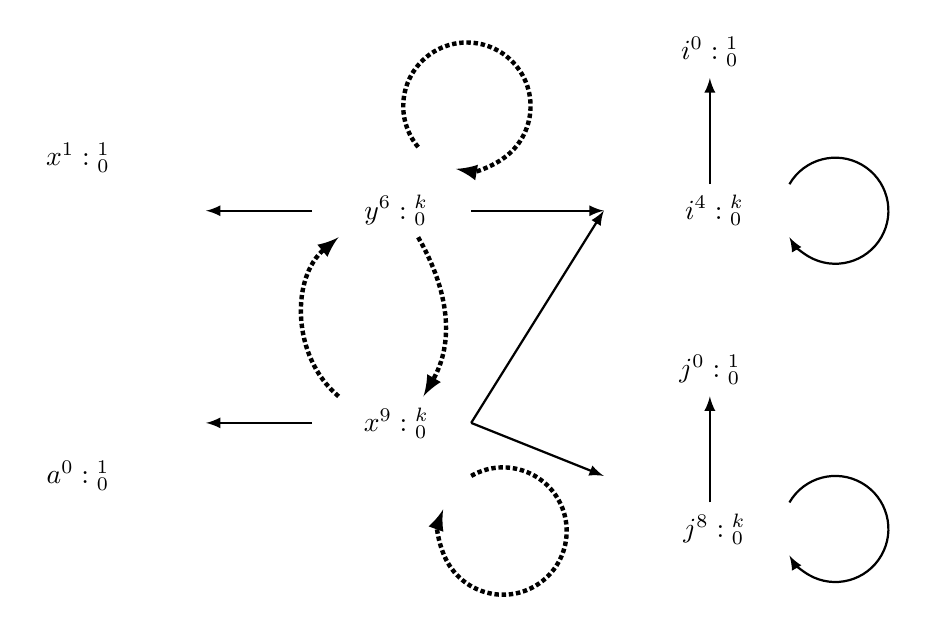
\begin{tikzpicture}[scale=\textwidth/18cm,samples=200]
% Variables Initialization
\draw[] (-6, 1) circle (0pt) node{{ $a^0: {}^1_{0}$}};
\draw[] (-6, 7) circle (0pt) node{{ $x^1: {}^{1}_{0}$}};
% Variables Inside the Loop
   \draw[] (0, 6) circle (0pt) node{{ $y^6: {}^{k}_{0}$}};
   \draw[] (0, 2) circle (0pt) node{{ $x^9: {}^{k}_{0}$}};
   % Counter Variables
   \draw[] (6, 9) circle (0pt) node {{$i^0: {}^{1}_{0}$}};
   \draw[] (6, 6) circle (0pt) node {{ $i^4: {}^{k}_{0}$}};
   \draw[] (6, 3) circle (0pt) node {{$j^0: {}^{1}_{0}$}};
   \draw[] (6, 0) circle (0pt) node {{ $j^8: {}^{k}_{0}$}};
   %
   % Value Dependency Edges:
   \draw[ ultra thick, -latex, densely dotted,] (0.5, 7.2) arc (220:-100:1.2);
   \draw[ thick, -latex] (6, 6.5)  -- (6, 8.5) ;
   \draw[ thick, -latex] (6, 0.5)  -- (6, 2.5) ;
   \draw[ ultra thick, -latex, densely dotted,] (1.5, 1.0) arc (120:-200:1.2);
   % Value Dependency Edges on Initial Values:
   \draw[ thick, -latex,] (-1.5, 2)  -- (-3.5, 2) ;
   \draw[ thick, -latex,] (-1.5, 6)  -- (-3.5, 6) ;
   %
   \draw[ ultra thick, -latex, densely dotted,] (-1, 2.5)  to  [out=-220,in=220]  (-1, 5.5);
   \draw[ ultra thick, -latex, densely dotted,]  (0.5, 5.5) to  [out=-60,in=60] (0.6, 2.5) ;
   % Control Dependency
  %  \draw[ thick,-latex] (1.5, 7)  -- (4, 9) ;
  %  \draw[ thick,-latex] (1.5, 4)  -- (4, 9) ;
  \draw[ thick, -latex, ] (7.5, 6.5) arc (150:-150:1);
  \draw[ thick, -latex, ] (7.5, 0.5) arc (150:-150:1);
  \draw[ thick,-latex] (1.5, 6)  -- (4, 6) ;
   \draw[ thick,-latex] (1.5, 2)  -- (4, 6) ;
   \draw[ thick,-latex] (1.5, 2)  -- (4, 1) ;
   \end{tikzpicture}
   \caption{}
      \end{centering}
      \end{subfigure}
    }
    % \end{wrapfigure}
    % \end{equation*}
    \vspace{-0.4cm}
     \caption{(a) The nested while loop example, (b) The program-based dependency graph generated from $\THESYSTEM$.}
    \label{fig:alg_adaptsearch_nestedwhile}
    \vspace{-0.7cm}
    \end{figure}
    %
        \begin{algorithm}
          \caption{
          {Over-Approximated Adaptivity on SCC}
          \label{alg:overadp_alg}
          }
          \begin{algorithmic}[1]
          \REQUIRE $G = (\vertxs, \edges, \weights, \qflag)$ \#\{An Strong Connected Symbolic Weighted Directed Graph\}
          \STATE {\bf {$\kw{\pathsearch_{scc-naive}(G)}$}:}  
          \STATE {\bf init} 
          \\
          $\kw{r_{scc}}$: the Adaptivity of this SCC
          \STATE  {\bf for} every vertex $v$ in $\vertxs$:
          \STATE  \qquad $\kw{r_{scc}} += \weights(v)*\qflag(v)$  
          \RETURN $r[c]$
          \end{algorithmic}
          \end{algorithm}
          %